\documentclass[../differential_methods.tex]{subfiles}
\begin{document}
\section{Aula 11 - 20 de Abril, 2026}
\subsection{Motivações}
\begin{itemize}
	\item Métodos de Runge-Kutta
\end{itemize}
\begin{example}[Estabilidade do Método de Euler Implícito]
	Para o método implícito, temos
	\[
		\lim_{n\to \infty}U^{n} = 0 \Longleftrightarrow | 1-z | > 1,
	\]
	onde \(z = h\lambda , \lambda \in \mathbb{C}\).

	Logo, em contraste ao explícito, a região de estabilidade do método de Euler implícito é a região exterior ao disco de centro em 1 e raio 1:
	\begin{figure}[H]
		\begin{center}
			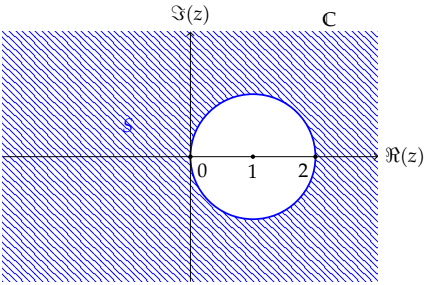
\includegraphics[height=0.6\textheight, width=0.6\textwidth, keepaspectratio]{./Images/ros_ieuler_10.png}
		\end{center}
	\end{figure}
\end{example}
\begin{example}[Estabilidade do Método do Trapézio]
	Sendo \(\lambda \in \mathbb{C}\), temos
	\[
		\lim_{n\to \infty}U^{n} = 0 \Longleftrightarrow \biggl\vert \frac{1+\frac{z}{2}}{1-\frac{z}{2}} \biggr\vert < 1,
	\]
	que acontece apenas quando \(\mathrm{Re}(z) < 0\).

	Desse modo, a região de estabilidade do método do trapézio é todo o lado esquerdo do plano complexo:
	\begin{figure}[H]
		\begin{center}
			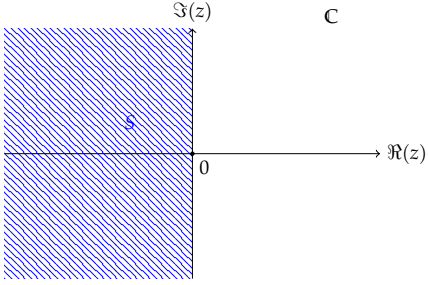
\includegraphics[height=0.6\textheight, width=0.6\textwidth, keepaspectratio]{./Images/ros_trapezoidal_10.png}
		\end{center}
	\end{figure}
\end{example}

Considere agora um sistema linear de EDO's dado por
\[
	\mathbf{u}'(t) = A \mathbf{u}(t), \quad \mathbf{u}(0) = \underline{\lambda} ,
\]
onde \(A\in \mathbb{R}^{m\times m}\) é constante e diagonalizável.

Como ela é diagonalizável, existem m autovetores linearmente independentes para a matriz A; denotando-os por \(\mathbf{v}^{i}\), eles são associados a m autovalores \(\lambda_{i}\in \mathbb{C}\), tal que
\[
	A \mathbf{v}^{i} = \lambda_{i}\mathbf{v}^{i}, \quad i=1, \dotsc , m.
\]
Seja, também, \(R = [\mathbf{v}^{1}, \mathbf{v}^{2}, \dotsc , \mathbf{v}^{m}]\) a matriz cujas colunas são os autovetores \(\mathbf{v}^{i}\), e \(\Lambda \) uma matriz diagonal com os autovalores \(\lambda_{i}\), de forma que a diagonalizabilidade de A permite escrevermos
\[
	A = R \Lambda R^{-1}
\]
e, assim,
\[
	\Lambda  = R^{-1}AR.
\]

Portanto, faz sentido definir a transformação linear
\[
	\mathbf{v}(t) = R^{-1}\mathbf{u}(t) \Rightarrow \mathbf{v}'(t)=R^{-1}\mathbf{u}'(t),
\]
tal que
\begin{align*}
	            & \mathbf{u}'(t) = A \mathbf{u}(t)                    \\
	\Rightarrow & R^{-1}\mathbf{u}'(t) = R^{-1}ARR^{-1} \mathbf{u}(t) \\
	\Rightarrow & \mathbf{v}'(t) = R^{-1}AR \mathbf{v}(t)             \\
	\Rightarrow & \mathbf{v}'(t) = \Lambda \mathbf{v}(t),
\end{align*}
transformando o sistema de EDO's no sistema desacoplado
\[
	v_{j}'(t) = \lambda_{j} v_{j}(t), \quad j=1, 2, \dotsc , m.
\]
\begin{def*}
	Um método geral de um passo é dito \textbf{absolutamente estável} para um sistema linear da forma
	\[
		\mathbf{u}'(t) = A \mathbf{u}(t), \quad \mathbf{u}(0) = \underline{\lambda },
	\]
	onde A é uma matriz m por m real e diagonalizável, se \(z_{j} = h\lambda_{j}\in S\) para todos os autovalores \(\lambda_{j}\) da matriz A, qualquer que seja a escolha de \(h > 0.\)

	Caso haja uma condição sobre h para que essa condição seja satisfeita, o método é dito \textbf{condicionalmente estável}. \(\square\)
\end{def*}
\begin{example}
	Considere o sistema de EDOs rígidas
	\begin{align*}
		 & u_{1}^{'} = -5u_1 + 3u_2     \\
		 & u_{2}^{'} = 100u_1 - 301u_2,
	\end{align*}
	que pode ser reescrito como
	\[
		u'(t) = \begin{bmatrix}
			-5  & 3    \\
			100 & -301
		\end{bmatrix} u(t)
	\]
	Quando decompomos o espectro, é como se saíssemos de um problema de um monte de ondas acopladas para suas componentes individuais! Os autovalores \(\lambda_1, \lambda_2\) dessa matriz serão usados, então, para determinar a região de estabilidade absoluta por meio de
	\[
		| 1+\lambda_1 h | < 1 \quad\&\quad | 1+ \lambda_2 h | < 1.
	\]
\end{example}

Para sistemas não lineares, como \(u' = f(u)\), a análise de estabilidade vista até agora falha em ser aplicada; no entanto, se a solução variar lentamente em relação aos passos temporais, então podemos linearizar ele de forma aproximada dentro do intervalo para ter uma noção decente do que está acontecendo:
\[
	u'(t) = f(u(t)) = f(v(t) + \overline{u}),
\]
onde a linearização foi do tipo \(u(t) = v(t) + \overline{u},\; u'(t) = v'(t)\).

Daí, expandindo em Taylor em torno de v(t) à ordem 2,
\[
	v'(t) = f(\overline{u}) + f'(\overline{u})v(t) + \mathcal{O}(\Vert v \Vert^{2}),
\]
tal que, derrubando o termo do erro, obtemos o sistema linear
\[
	v'(t) = A v(t) + b,
\]
sendo \(A = f'(\overline{u})\) a matriz Jacobiana avaliada em \(\overline{u}\), e \( b = f(\overline{u})\).

Desta forma, examinar como esse método numérico se comporta para esse sistema linear em cada valor relevante de \(\overline{u}\) fornece uma boa ideia de como ele se comportará no caso do sistema não linear também!
O problema é que, se houver uma região de não linearidade muito súbita ou intensa, esse método de linearização falha!

\begin{example}
	Vamos considerar o exemplo do pêndulo
	\[
		\left\{\begin{array}{ll}
			u_{1}^{'}(t) = u_2(t) \\
			u_{2}^{'}(t) = -\sin^{}{(u_1(t))}
		\end{array}\right..
	\]
	Pelo que vimos, precisamos calcular a matriz jacobiana associada à função \(f(u(t)) = (u_2(t), -\sin^{}{(u_1(t))})\) desse sistema:
	\[
		A = \frac{\partial^{}f}{\partial u^{}} = \begin{pmatrix}
			\frac{\partial^{}f_1}{\partial u_1^{}} & \frac{\partial^{}f_1}{\partial u_2^{}} \\
			\frac{\partial^{}f_2}{\partial u_1^{}} & \frac{\partial^{}f_2}{\partial u_2^{}}
		\end{pmatrix} = \begin{pmatrix}
			0                  & 1 \\
			-\cos^{}{(u_1(t))} & 0
		\end{pmatrix}
	\]
	Queremos saber se o problema, com a matriz jacobiana, é estável; quanto aos autovalores, temos
	\begin{align*}
		\det{(A - \lambda I)} = 0 & \Rightarrow \det\begin{bmatrix}
			                                            -\lambda           & 1        \\
			                                            -\cos^{}{(u_1(t))} & -\lambda
		                                            \end{bmatrix} = 0          \\
		                          & \Rightarrow \lambda^{2} + \cos^{}{(u_1(t))} = 0        \\
		                          & \Rightarrow \lambda  = \pm \sqrt[]{-\cos^{}{(u_1(t))}}
	\end{align*}
	Fixando no intervalo \(\displaystyle \biggl[-\frac{\pi }{2}, \frac{\pi }{2}\biggr]\) por sua utilidade física, o cosseno é sempre positivo e os autovalores serão sempre da forma
	\[
		\lambda = \pm i \sqrt[]{\cos^{}{(u_1(t))}},
	\]
	ou seja, se quiséssemos resolver o pêndulo com o método de Euler para a solução não explodir catastroficamente, precisaríamos de um h tal que \(| 1+\lambda_{i}h | < 1\)... O problema é que não existe h que satisfaça isso! O método de Euler não funciona!!

	Portanto, a conclusão é: \textbf{não use o método de Euler}.
\end{example}
\begin{tcolorbox}[
		skin=enhanced,
		title=Observação,
		fonttitle=\bfseries,
		colframe=black,
		colbacktitle=cyan!75!white,
		colback=cyan!15,
		colbacklower=black,
		coltitle=black,
		drop fuzzy shadow,
		%drop large lifted shadow
	]
	Quando vimos a aproximação com o método de Euler, não foi o caso dela explodir catastroficamente, e o motivo para essa ``inconsistência'' com a análise acima é que o termo de erro pode sim incluir alguns pontos onde o método não irá explodir; porém, visando sempre \textbf{\textit{reduzir os erros}}, a escolha menos errada é não utilizar o método de Euler para não depender dessa sorte!
\end{tcolorbox}


\subsection{Métodos Runge-Kutta Explícitos}
Até o momento, estivemos usando o método de Taylor para as nossas aproximações, e já vimos alguns dos problemas que ele tem. Será que existem métodos diferentes para aproximar nossas equações
A ideia é que sim, existem outros, e veremos um deles a seguir: o método de Runge-Kutta, que também tem suas versões explícita e implícita, mas focaremos apenas na primeira.

Quando utilizamos o método de Euler explícito, existe uma ideia geométrica que faz uso de retas conectando os valores por trás dos panos:
\begin{figure}[H]
	\begin{center}
		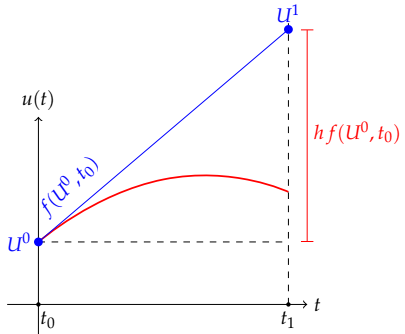
\includegraphics[height=0.6\textheight, width=0.6\textwidth, keepaspectratio]{./Images/geometric_euler_11.png}
	\end{center}
\end{figure}
Porém, e se utilizarmos um monte de inclinações intermediárias para chegar à final? O custo certamente aumentará, mas ganharemos um tanto de precisão! Para isso, utilizamos
\[
	U^{n+1} = U^{n} + h \varphi (U^{n}, t_{n}, h),
\]
com
\[
	\varphi (U^{n}, t_{n}, h) = \sum\limits_{j}^{}b_{j}f(Z^{j}, t_{k_{j}}),
\]
onde \(t_{k_{j}}\) são os passos intermediários entre \(t_{j-1}\) e \(t_{j}\): aumentamos a ordem de precisão calculando inclinações em passos intermediários, e é essa a ideia dos \textit{métodos tipo Runge-Kutta}
\begin{figure}[H]
	\begin{center}
		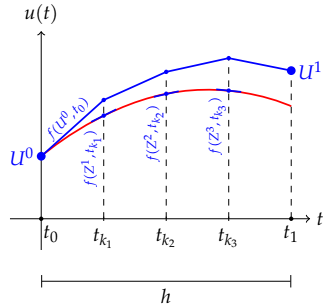
\includegraphics[height=0.6\textheight, width=0.6\textwidth, keepaspectratio]{./Images/intermediate_steps_11.png}
	\end{center}
\end{figure}

A forma geral dos \textbf{Métodos Runge-Kutta Explícitos de R Estágios} é:
\begin{align*}
	 & \mathbf{K}^{1} = \mathbf{f}(\mathbf{U}^{n}, t_{n})                                                                       \\
	 & \mathbf{K}^{2} = \mathbf{f}(\mathbf{U}^{n}+ha_{21}\mathbf{K}^{1}, t_{n}+hc_{2})                                          \\
	 & \mathbf{K}^{3} = \mathbf{f}(\mathbf{U}^{n} + h a_{31}\mathbf{K}^{1} + h a_{32} \mathbf{K}^{2}, t_{n} + h c_{3})          \\
	 & \vdots                                                                                                                   \\
	 & \mathbf{K}^{R}=\mathbf{f}\biggl(\mathbf{U}^{n} + h \sum\limits_{j=1}^{R-1}a_{R_{j}}\mathbf{K}^{j}, t_{n}+ h c_{R}\biggr) \\
	 & \mathbf{U}^{n+1} = \mathbf{U}^{n} + h \sum\limits_{j=1}^{R}b_{j}K^{j},
\end{align*}
de forma que o método é completamente determinado pelo coeficientes \(a_{ij},\; b_{j}\) e \(c_{j}\), que não são determinadas exatamente e precisam ser determinadas ao longo do método!

Como foi deixado bem aparente, dá para fazer uma representação dessa classe de métodos com matrizes:
\begin{table}[H]
	\centering
	\begin{tabular}{c | c c c c c}
		0          & 0          &            &             &                &           \\
		\(c_2\)    & \(a_{21}\) & 0          &             &                &           \\
		\(c_3\)    & \(a_{31}\) & \(a_{32}\) & 0           &                &           \\
		\(\vdots\) & \(\vdots\) & \(\vdots\) & \(\ddots\)  & \(\ddots\)     &           \\
		\(c_{R}\)  & \(a_{R1}\) & \(a_{R2}\) & \(\dotsc\)  & \(a_{R, R-1}\) & 0         \\
		\hline
		           & \(b_1\)    & \(b_2\)    & \(\dotsc \) & \(b_{R_1}\)    & \(b_{R}\)
	\end{tabular}
\end{table}

Ou, de forma mais curta,
\begin{table}[H]
	\centering
	\begin{tabular}{c | c}
		\(\mathbf{c}\) & \(\mathbf{A}\)     \\
		\hline
		               & \(\mathbf{b}^{t}\)
	\end{tabular}
\end{table}
onde \(\mathbf{A}\) é uma matriz triangular inferior com diagonal nula e \(c_{1} = 0\).

Um \textbf{método RK de 1 estágio} é simplificado da forma geral e dado por
\[
	\boxed{\mathbf{U}^{n+1} = \mathbf{U}^{n} + h b_{1}\mathbf{f}(\mathbf{U}^{n}, t_{n})}
\]
É basicamente um método de Euler.
\begin{tcolorbox}[
		skin=enhanced,
		title=Observação,
		fonttitle=\bfseries,
		colframe=black,
		colbacktitle=cyan!75!white,
		colback=cyan!15,
		colbacklower=black,
		coltitle=black,
		drop fuzzy shadow,
		%drop large lifted shadow
	]
	Nesse ponto, já deu pra perceber que o método de Euler é basicamente um elemento neutro dos métodos numéricos :p
\end{tcolorbox}

Quanto ao seu erro de truncamento,
\begin{align*}
	\tau^{n} & = \frac{1}{h}(\mathbf{u}(t_{n+1}) - \mathbf{u}(t_{n})) - b_1 \mathbf{f}(\mathbf{u}(t_{n}), t_{n})                                                                                 \\
	         & = \frac{1}{h}\biggl(\mathbf{u}(t_{n}) + h \mathbf{u}'(t_{n}) + \frac{h^{2}}{2} \mathbf{u}''(t_{n}) + \dotsc - \mathbf{u}(t_{n})\biggr) - b_1 \mathbf{f}(\mathbf{u}(t_{n}), t_{n}) \\
	         & = (1-b_1)\mathbf{u}'(t_{n}) + \frac{h}{2}\mathbf{u}''(t_{n}) + \dotsc
\end{align*}
Logo, para que o método seja consistente de ordem \(\mathcal{O}(h)\), devemos ter \(b_1 = 1.\)

A forma geral dos \textbf{métodos RK de 2 estágios} é
\begin{align*}
	 & \mathbf{K}^{1} = \mathbf{f}(\mathbf{U}^{n}, t_{n})                               \\
	 & \mathbf{K}^{2} = \mathbf{f}(\mathbf{U}^{n} + h a_{21}\mathbf{K}^{1}, t_{n}+hc_2) \\
	 & \mathbf{U}^{n+1} = \mathbf{U}^{n} + h (b_1 \mathbf{K}^{1} + b_2 \mathbf{K}^{2}),
\end{align*}
tal que, substituindo \(\mathbf{K}^{1}\) e \(\mathbf{K}^{2}\), obtemos
\[
	\boxed{\mathbf{U}^{n+1} = \mathbf{U}^{n} + h \{\underbrace{b_1 \mathbf{f}(\mathbf{U}^{n}, t_{n}) + b_2 \mathbf{f}(\mathbf{U}^{n} + h a_{21}\mathbf{f}(\mathbf{U}^{n}, t_{n}), t_{n}+ h c_2)}_{\varphi (\mathbf{U}^{n}, t_{n}, h)}\}}
\]
Calculando o erro de truncamento,
\begin{align*}
	\tau^{n} & = \frac{1}{h}(\mathbf{u}(t_{n+1}) - \mathbf{u}(t_{n})) - b_1 \mathbf{f}(\mathbf{u}(t_{n}), t_{n})                                                                                                                                                                                                                                             \\
	         & - b_2 \mathbf{f}\biggl(\underline{\mathbf{u}(t_{n})+ha_{21}\mathbf{f}(\mathbf{u}(t_{n}), t_{n})}, \underline{t_{n}+hc_2}\biggr)                                                                                                                                                                                                               \\
	         & = \frac{1}{h}\biggl(\mathbf{u}(t_{n}) + h \mathbf{u}'(t_{n}) + \frac{h^{2}}{2}\mathbf{u}''(t_{n}) + \dotsc - \mathbf{u}(t_{n})\biggr) - b_1 \mathbf{u}'(t_{n})                                                                                                                                                                                \\
	         & - b_2 \biggl\{\mathbf{f}(\mathbf{u}(t_{n}), t_{n}) + h a_{21}\frac{\partial^{}\mathbf{f}}{\partial \mathbf{u}^{}}\mathbf{f}\biggl|_{\mathrlap{(\mathbf{u}(t_{n}), t_{n})}}^{}\biggr. +\;\; h c_2 \frac{\partial^{}\mathbf{f}}{\partial t^{}}\biggl|_{\mathrlap{(\mathbf{u}(t_{n}), t_{n})}}^{}\biggr. +\;\; \dotsc \biggr\}                   \\
	         & = (1-b_1-b_2)\mathbf{u}'(t_{n}) + h \biggl(\frac{1}{2}\mathbf{u}''(t_{n}) - b_2a_{21}\frac{\partial^{}\mathbf{f}}{\partial \mathbf{u}^{}}\mathbf{f}\biggl|_{\mathrlap{(\mathbf{u}(t_{n}), t_{n}}}^{}\biggr. \;-\; b_2c_2 \frac{\partial^{}\mathbf{f}}{\partial t^{}}\biggl|_{(\mathbf{u}(t_{n}), t_{n})}^{}\biggr.\biggr)+\mathcal{O}(h^{2}).
\end{align*}

Portanto, o método de 2 estágio será consistente apenas se
\[
	\left\{\begin{array}{ll}
		b_1 + b_2 = 1 \\
		a_{21} = c_2  \\
		b_2c_2 = \frac{1}{2}
	\end{array}\right.,
\]
que é um sistema não linear com 3 equações e 4 incógnitas, ou seja, com infinitas soluções. Desta forma, existem infinitos métodos Runge-Kutta explícitos de dois estágios que são consistentes e de ordem \(\mathcal{O}(h^{2})\).

\begin{example}[Modificando o Método de Euler]
	O \textbf{método de Euler modificado} é dado pelos coeficientes de Runge-Kutta da forma
	\begin{table}[H]
		\centering
		\begin{tabular}{c | c c}
			0               & 0               &   \\
			\(\frac{1}{2}\) & \(\frac{1}{2}\) & 0 \\
			\hline
			                & 0               & 1
		\end{tabular}
	\end{table},
	que leva ao sistema
	\[
		\left\{\begin{array}{ll}
			\mathbf{K}^{1} = \mathbf{f}(\mathbf{U}^{n}, t_{n})                                                     \\
			\mathbf{K}^{2} = \mathbf{f}\bigl(\mathbf{U}^{n} + \frac{h}{2} \mathbf{K}^{1}, t_{n}+ \frac{h}{2}\bigr) \\
			\mathbf{U}^{n+1} = \mathbf{U}^{n} + h \mathbf{K}^{2}
		\end{array}\right..
	\]

	\pagebreak
	Além desse, o \textbf{método de Euler melhorado} tem a forma
	\begin{table}[H]
		\centering
		\begin{tabular}{c | c c}
			0 & 0               &                 \\
			1 & 1               & 0               \\
			\hline
			  & \(\frac{1}{2}\) & \(\frac{1}{2}\)
		\end{tabular},
	\end{table}
	que leva ao sistema
	\[
		\left\{\begin{array}{ll}
			\mathbf{K}^{1} = \mathbf{f}(\mathbf{U}^{n}, t_{n})                                \\
			\mathbf{K}^{2} = \mathbf{f}\bigl(\mathbf{U}^{n} + h\mathbf{K}^{1}, t_{n}+ h\bigr) \\
			\mathbf{U}^{n+1} = \mathbf{U}^{n} + \frac{h}{2} (\mathbf{K}^{1} + \mathbf{K}^{2})
		\end{array}\right..
	\]
\end{example}

Conforme o número de estágios aumenta, a ordem também aumenta:
\begin{itemize}
	\item 3 Passos (R=3): sistema de 4 equações e 6 incógnitas, resultando em \(\mathcal{O}(h^{3})\);
	\item 4 Passos (R=4): sistema de 11 equações e 13 incógnitas, resultando em \(\mathcal{O}(h^{4})\);
	\item \(\dotsc \)
\end{itemize}

De fato, é possível mostrar que a ordem p em função de R satisfaz a relação:
\begin{table}[H]
	\centering
	\begin{tabular}{c | c c c c c c c c c}
		R    & 1 & 2 & 3 & 4 & 5 & 6 & 7 & 8 & 9 \\
		\hline
		p(R) & 1 & 2 & 3 & 4 & 4 & 5 & 6 & 6 & 7 \\
	\end{tabular},
\end{table}
e, do estágio 10 adiante, temos a relação \(p(R)\leq R-2\).

Disso, tiramos que ele é um método explícito muito preciso, comparável aos métodos de Taylor e, mais importante, \textbf{não depende da diferenciabilidade de f}. Porém, ele tem um custo elevado, associado às sucessivas avaliações de f.
\begin{example}[Alguns Métodos de Runge-Kutta]
	Um exemplo para 3 estágios é o \textbf{Método RK3 de Heun}:
	\begin{table}[H]
		\centering
		\begin{tabular}{c | c c c}
			0               & 0               &                 &                 \\
			\(\frac{1}{3}\) & \(\frac{1}{3}\) & 0               &                 \\
			\(\frac{2}{3}\) & 0               & \(\frac{2}{3}\) & 0               \\
			\hline
			                & \(\frac{1}{4}\) & 0               & \(\frac{3}{4}\)
		\end{tabular},
	\end{table}
	com sistema
	\[
		\left\{\begin{array}{ll}
			\mathbf{K}^{1} = \mathbf{f}(\mathbf{U}^{n}, t_{n})                                                      \\
			\mathbf{K}^{2} = \mathbf{f}\bigl(\mathbf{U}^{n} + \frac{h}{3}\mathbf{K}^{1}, t_{n}+ \frac{h}{3}\bigr)   \\
			\mathbf{K}^{3} = \mathbf{f}\bigl(\mathbf{U}^{n} + \frac{2h}{3}\mathbf{K}^{2}, t_{n}+ \frac{2h}{3}\bigr) \\
			\mathbf{U}^{n+1} = \mathbf{U}^{n} + \frac{h}{4} (\mathbf{K}^{1} + 3\mathbf{K}^{3})
		\end{array}\right..
	\]

	Um exemplo para 4 estágios é o \textbf{Método RK4 Clássico/``O Método Runge-Kutta''}:
	\begin{table}[H]
		\centering
		\begin{tabular}{c | c c c c}
			0               & 0               &                 &                 &                 \\
			\(\frac{1}{2}\) & \(\frac{1}{2}\) & 0               &                 &                 \\
			\(\frac{1}{2}\) & 0               & \(\frac{1}{2}\) & 0               &                 \\
			1               & 0               & 0               & 1               & 0               \\
			\hline
			                & \(\frac{1}{6}\) & \(\frac{1}{3}\) & \(\frac{1}{3}\) & \(\frac{1}{6}\)
		\end{tabular},
	\end{table}
	com sistema
	\[
		\left\{\begin{array}{ll}
			\mathbf{K}^{1} = \mathbf{f}(\mathbf{U}^{n}, t_{n})                                                    \\
			\mathbf{K}^{2} = \mathbf{f}\bigl(\mathbf{U}^{n} + \frac{h}{2}\mathbf{K}^{1}, t_{n}+ \frac{h}{2}\bigr) \\
			\mathbf{K}^{3} = \mathbf{f}\bigl(\mathbf{U}^{n} + \frac{h}{2}\mathbf{K}^{2}, t_{n}+ \frac{h}{2}\bigr) \\
			\mathbf{K}^{4} = \mathbf{f}\bigl(\mathbf{U}^{n} + \mathbf{K}^{2}, t_{n}+ h\bigr)                      \\
			\mathbf{U}^{n+1} = \mathbf{U}^{n} + \frac{h}{6} (\mathbf{K}^{1} + 2\mathbf{K}^{2} + 2 \mathbf{K}^{3} + \mathbf{K}^{4})
		\end{array}\right..
	\]

	\begin{listing}[H]
		\caption{Implementação do RK4 para Presa-Predador}
		\begin{minted}[bgcolor = bg, linenos=true, breaklines]{Matlab}
 function fd = f_pp ( u)

 fd (1 ,1) = -2* u (1) + u (1) *u (2) ;
 fd (1 ,2) = u (2) - u (1) * u (2) ;

 ...
 while tn < tfim

   k1 = f_pp ( un ) ;
   k2 = f_pp ( un + h /2 * k1 );
   k3 = f_pp ( un + h /2 * k2 );
   k4 = f_pp ( un + k3 );
  
   un1 = un + h /6 * ( k1 + 2* k2 + 2* k3 + k4 );
  
   tn = tn + h;
   un = un1 ;

 end
 ...
 \end{minted}
	\end{listing}
\end{example}

\end{document}
